%%%%%%%%%%%%%%%%%%%%%%%%%%%%%%%%%%%%%%%%%%%%%%%%%%%%%%%%%%%%%%%%%%
% Integrantes:													 %
% 			- Adel Arja											 %
% 			- Santiago Nolasco									 %
% 			- Luis Guanuco										 %
% 																 %
% Fecha:		mié ago 26 20:01:26 ART 2015					 %
% 																 %
% Versión:	0.1													 %
% 																 %
% Nombre del proyecto:	TOKEN_IUA_ANG							 %
% 																 %
% Descripción: Se genera el documento con los requerimientos del %
% proyecto. En principio se realiza un borrador.				 %
%%%%%%%%%%%%%%%%%%%%%%%%%%%%%%%%%%%%%%%%%%%%%%%%%%%%%%%%%%%%%%%%%%
\documentclass[oneside,11pt,a4paper,spanish]{article}
%%%%%%%%%%%%
% Paquetes %
%%%%%%%%%%%%
\usepackage[utf8]{inputenc}
\usepackage[a4paper]{geometry}
\usepackage{graphicx}
\usepackage[spanish]{babel}

%%%%%%%%%%%%%
% Metadatos %
%%%%%%%%%%%%%

\title{Seguridad en la Información\\
\normalsize{Trabajo Práctico -- Requerimientos}}

\author{
Adel Arja \and
Santiago Nolasco \and
Luis Guanuco\footnote{contacto: \texttt{guanucoluis@gmail.com}}}

\date{\today}

\begin{document}

\maketitle

\begin{abstract}
  Se trabajará sobre la propuesta denominada \emph{TOKER\_IUA}. En
  esta primera entrega se comparten los requerimientos que demandará
  el proyecto. La figura que acompaña al final del documento
  complementa el texto.
\end{abstract}

\section{Requerimientos}

\begin{enumerate}
\item Se utilizará un sistema embebidos de bajo costo y una computadora
de escritorio (PC) como dispositivos principales que se comunicarán
entre sí.
\item El dispositivo embebido recibirá de la PC, mediante una
comunicación serial, un archivo (mensaje) y al mismo se le aplicarán
técnicas/algoritmos para conservar:
\begin{itemize}
\item Confidencialidad
\item Autenticidad
\item Integridad
\end{itemize}
el nuevo mensaje generado en el sistema embebido será devuelto a la
PC. Dónde se comprobarán que se hayan mantenido los items anteriores.
\begin{enumerate}
\item La confidencialidad del mensaje se realiza con alguna técnica de
encriptación a definir.
\item Se autenticará el mensaje utilizando el concepto de "firmas
digitales". Se definirán claves públicas y privadas de los
dispositivos que participan de la comunicación.
\item La integridad del mensaje se mantiene utilizando técnicas de
digesto.
\end{enumerate}
\end{enumerate}

\newpage{}
\section{Análisis y Diseño}

Cómo primera alternativa se evalúa la siguiente arquitectura a implementar.

\begin{figure}[h]
  \centering
  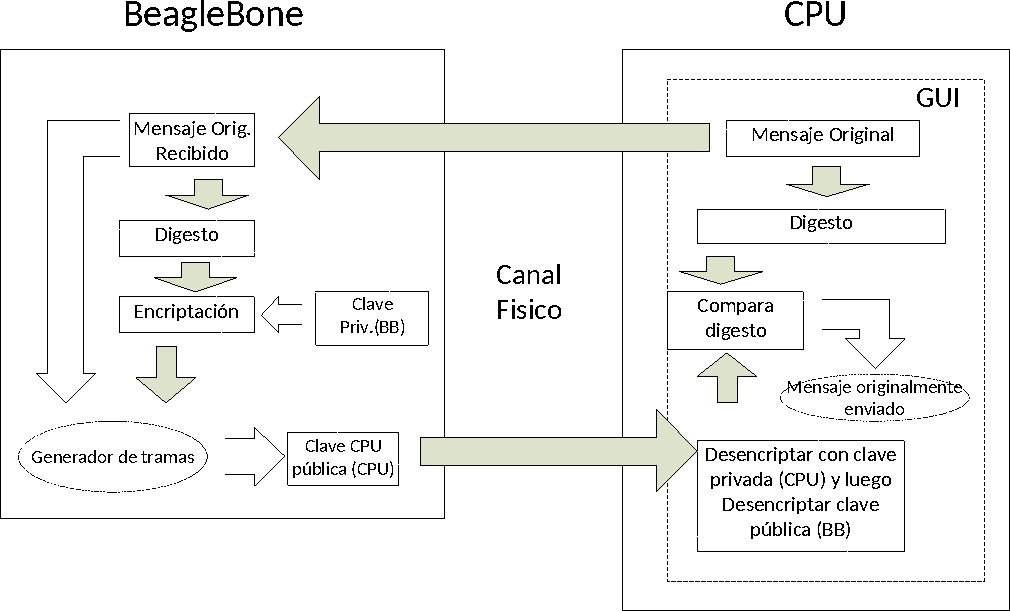
\includegraphics[width=\textwidth]{images/arch}
  \caption{Diagrama general del sistema a implementar.}
\end{figure}

\end{document}



